This section serves the testing of Hypothesis \ref{hpt:hypothesis_h} under
state of the global localisation art methods and CBGL, in varying environmental
conditions and sensor configurations. With regard to CBGL its three required
parameters are set to $(d_{\bm{l}},d_{\alpha},k) = (40, 2^5, 10)$ after
initial tests with the dataset used in subsection \ref{subsec:exp_a}.
The rationale of choosing appropriate $d_{\bm{l}},d_{\alpha}$ is depicted in
figure \ref{fig:a:determine_40_32}, and $k$ is chosen as such in order to
retain a high-enough true positive discovery rate without significant increase
in execution time.
%(due to the application of scan--to--map-scan matching on $k$
%pose estimates).
References to sets $\mathcal{H}_{\ast}$ are made to fig. \ref{fig:block_system}
(left) and lines \ref{alg:cbgl:h}, \ref{alg:cbgl:h1}, and \ref{alg:cbgl:h2} of
Algorithm \ref{alg:cbgl}. All tests were performed with a processor of 12
threads and a clock speed of 4.00 GHz.


%%%%%%%%%%%%%%%%%%%%%%%%%%%%%%%%%%%%%%%%%%%%%%%%%%%%%%%%%%%%%%%%%%%%%%%%%%%%%%%%
\subsection{Experiments in real conditions}
\label{subsec:exp_a}

The first type of test is conducted with the use of a Hokuyo UTM-30LX
sensor, whose angular range is $\lambda = 3\pi/2$ rad and radial range
$r_{\max} = 30.0$ m, in the  Electrical and Computer Engineering Department's
Laboratory of Computer Systems Architecture (CSAL), Aristotle University of
Thessaloniki, Greece, a map of which is depicted in figure
\ref{fig:a:map_and_trajectory}. The sensor was mounted on a Robotnik RB1 robot,
which was teleoperated within the environment while scans were being recorded.
This resulted in $N_{S}=6669$ range scans, whose number of rays are downsampled
by a factor of four before being inputted to CBGL and ALS \cite{als_jp}, an
algorithm which implements Free-Space Features \cite{als_eth}. Other global
localisation methods are not to tested for this type of experiment due to
their infeasible execution time with respect to the range dataset's volume (see
fig. \ref{fig:b:execution_times}). CBGL's internal \texttt{sm2}
method is chosen to be PLICP \cite{Censi2008c} due to its low execution time
and the sensor's non-panoramic field of view. The top of figure
\ref{fig:a:awesomeness} depicts the proportion of output pose estimates from
each method whose position and orientation error is lower than outlier
thresholds $\delta_{\bm{l}}$, $\delta_{\theta}$; at the bottom they are
depicted exclusively with regard to CBGL's output and its internal pose sets.
The mean and standard deviation of the two methods' execution times are
$(\mu_t^{\text{ALS}}, \sigma_t^{\text{ALS}}) = (6.15, 5.32)$ sec, and
$(\mu_t^{\text{CBGL}}, \sigma_t^{\text{CBGL}}) = (1.61, 0.06)$ sec. From the
experimental evidence it is clear that (a) hypothesis \ref{hpt:hypothesis_h} is
observed to be true $991$ times out of a thousand for an outliers' locational
threshold $\delta_{\bm{l}} = 0.5$ m when an angular threshold is
$\delta_{\theta}$ is not considered, and (b) CBGL outperforms ALS in terms of
(i) number of pose estimates within all locational and angular thresholds and
(ii) execution time.

\begin{figure}
  \vspace{-0.3cm}
  % GNUPLOT: LaTeX picture with Postscript
\begingroup
  \makeatletter
  \providecommand\color[2][]{%
    \GenericError{(gnuplot) \space\space\space\@spaces}{%
      Package color not loaded in conjunction with
      terminal option `colourtext'%
    }{See the gnuplot documentation for explanation.%
    }{Either use 'blacktext' in gnuplot or load the package
      color.sty in LaTeX.}%
    \renewcommand\color[2][]{}%
  }%
  \providecommand\includegraphics[2][]{%
    \GenericError{(gnuplot) \space\space\space\@spaces}{%
      Package graphicx or graphics not loaded%
    }{See the gnuplot documentation for explanation.%
    }{The gnuplot epslatex terminal needs graphicx.sty or graphics.sty.}%
    \renewcommand\includegraphics[2][]{}%
  }%
  \providecommand\rotatebox[2]{#2}%
  \@ifundefined{ifGPcolor}{%
    \newif\ifGPcolor
    \GPcolorfalse
  }{}%
  \@ifundefined{ifGPblacktext}{%
    \newif\ifGPblacktext
    \GPblacktexttrue
  }{}%
  % define a \g@addto@macro without @ in the name:
  \let\gplgaddtomacro\g@addto@macro
  % define empty templates for all commands taking text:
  \gdef\gplfronttext{}%
  \gdef\gplfronttext{}%
  \makeatother
  \ifGPblacktext
    % no textcolor at all
    \def\colorrgb#1{}%
    \def\colorgray#1{}%
  \else
    % gray or color?
    \ifGPcolor
      \def\colorrgb#1{\color[rgb]{#1}}%
      \def\colorgray#1{\color[gray]{#1}}%
      \expandafter\def\csname LTw\endcsname{\color{white}}%
      \expandafter\def\csname LTb\endcsname{\color{black}}%
      \expandafter\def\csname LTa\endcsname{\color{black}}%
      \expandafter\def\csname LT0\endcsname{\color[rgb]{1,0,0}}%
      \expandafter\def\csname LT1\endcsname{\color[rgb]{0,1,0}}%
      \expandafter\def\csname LT2\endcsname{\color[rgb]{0,0,1}}%
      \expandafter\def\csname LT3\endcsname{\color[rgb]{1,0,1}}%
      \expandafter\def\csname LT4\endcsname{\color[rgb]{0,1,1}}%
      \expandafter\def\csname LT5\endcsname{\color[rgb]{1,1,0}}%
      \expandafter\def\csname LT6\endcsname{\color[rgb]{0,0,0}}%
      \expandafter\def\csname LT7\endcsname{\color[rgb]{1,0.3,0}}%
      \expandafter\def\csname LT8\endcsname{\color[rgb]{0.5,0.5,0.5}}%
    \else
      % gray
      \def\colorrgb#1{\color{black}}%
      \def\colorgray#1{\color[gray]{#1}}%
      \expandafter\def\csname LTw\endcsname{\color{white}}%
      \expandafter\def\csname LTb\endcsname{\color{black}}%
      \expandafter\def\csname LTa\endcsname{\color{black}}%
      \expandafter\def\csname LT0\endcsname{\color{black}}%
      \expandafter\def\csname LT1\endcsname{\color{black}}%
      \expandafter\def\csname LT2\endcsname{\color{black}}%
      \expandafter\def\csname LT3\endcsname{\color{black}}%
      \expandafter\def\csname LT4\endcsname{\color{black}}%
      \expandafter\def\csname LT5\endcsname{\color{black}}%
      \expandafter\def\csname LT6\endcsname{\color{black}}%
      \expandafter\def\csname LT7\endcsname{\color{black}}%
      \expandafter\def\csname LT8\endcsname{\color{black}}%
    \fi
  \fi
    \setlength{\unitlength}{0.0500bp}%
    \ifx\gptboxheight\undefined%
      \newlength{\gptboxheight}%
      \newlength{\gptboxwidth}%
      \newsavebox{\gptboxtext}%
    \fi%
    \setlength{\fboxrule}{0.5pt}%
    \setlength{\fboxsep}{1pt}%
\begin{picture}(4500.00,4000.00)%
    \gplgaddtomacro\gplfronttext{%
      \colorrgb{0.15,0.15,0.15}%
      \put(318,2666){\makebox(0,0)[r]{\strut{}\footnotesize $0$}}%
      \colorrgb{0.15,0.15,0.15}%
      \put(318,2899){\makebox(0,0)[r]{\strut{}\footnotesize $500$}}%
      \colorrgb{0.15,0.15,0.15}%
      \put(318,3133){\makebox(0,0)[r]{\strut{}\footnotesize $1000$}}%
      \colorrgb{0.15,0.15,0.15}%
      \put(318,3366){\makebox(0,0)[r]{\strut{}\footnotesize $1500$}}%
      \colorrgb{0.15,0.15,0.15}%
      \put(318,3599){\makebox(0,0)[r]{\strut{}\footnotesize $2000$}}%
      \colorrgb{0.15,0.15,0.15}%
      \put(498,2566){\makebox(0,0){\strut{}\scriptsize $0$}}%
      \colorrgb{0.15,0.15,0.15}%
      \put(688,2566){\makebox(0,0){\strut{}\scriptsize $2$}}%
      \colorrgb{0.15,0.15,0.15}%
      \put(879,2566){\makebox(0,0){\strut{}\scriptsize $4$}}%
      \colorrgb{0.15,0.15,0.15}%
      \put(1070,2566){\makebox(0,0){\strut{}\scriptsize $6$}}%
      \colorrgb{0.15,0.15,0.15}%
      \put(1261,2566){\makebox(0,0){\strut{}\scriptsize $8$}}%
      \colorrgb{0.15,0.15,0.15}%
      \put(1451,2566){\makebox(0,0){\strut{}\scriptsize $10$}}%
    }%
    \gplgaddtomacro\gplfronttext{%
      \colorrgb{0.15,0.15,0.15}%
      \put(974,3716){\makebox(0,0){\strut{}\footnotesize $d_{\alpha} = 2^3$}}%
    }%
    \gplgaddtomacro\gplfronttext{%
      \colorrgb{0.15,0.15,0.15}%
      \put(1592,2666){\makebox(0,0)[r]{\strut{}}}%
      \colorrgb{0.15,0.15,0.15}%
      \put(1592,2899){\makebox(0,0)[r]{\strut{}}}%
      \colorrgb{0.15,0.15,0.15}%
      \put(1592,3133){\makebox(0,0)[r]{\strut{}}}%
      \colorrgb{0.15,0.15,0.15}%
      \put(1592,3366){\makebox(0,0)[r]{\strut{}}}%
      \colorrgb{0.15,0.15,0.15}%
      \put(1592,3599){\makebox(0,0)[r]{\strut{}}}%
      \colorrgb{0.15,0.15,0.15}%
      \put(1772,2566){\makebox(0,0){\strut{}\scriptsize $0$}}%
      \colorrgb{0.15,0.15,0.15}%
      \put(1963,2566){\makebox(0,0){\strut{}\scriptsize $2$}}%
      \colorrgb{0.15,0.15,0.15}%
      \put(2154,2566){\makebox(0,0){\strut{}\scriptsize $4$}}%
      \colorrgb{0.15,0.15,0.15}%
      \put(2356,2566){\makebox(0,0){\strut{}\scriptsize $6$}}%
      \colorrgb{0.15,0.15,0.15}%
      \put(2535,2566){\makebox(0,0){\strut{}\scriptsize $8$}}%
      \colorrgb{0.15,0.15,0.15}%
      \put(2726,2566){\makebox(0,0){\strut{}\scriptsize $10$}}%
    }%
    \gplgaddtomacro\gplfronttext{%
      \colorrgb{0.15,0.15,0.15}%
      \put(2249,3716){\makebox(0,0){\strut{}\footnotesize $d_{\alpha} = 2^4$}}%
    }%
    \gplgaddtomacro\gplfronttext{%
      \colorrgb{0.15,0.15,0.15}%
      \put(3048,2566){\makebox(0,0){\strut{}\scriptsize $0$}}%
      \colorrgb{0.15,0.15,0.15}%
      \put(3238,2566){\makebox(0,0){\strut{}\scriptsize $2$}}%
      \colorrgb{0.15,0.15,0.15}%
      \put(3429,2566){\makebox(0,0){\strut{}\scriptsize $4$}}%
      \colorrgb{0.15,0.15,0.15}%
      \put(3620,2566){\makebox(0,0){\strut{}\scriptsize $6$}}%
      \colorrgb{0.15,0.15,0.15}%
      \put(3811,2566){\makebox(0,0){\strut{}\scriptsize $8$}}%
      \colorrgb{0.15,0.15,0.15}%
      \put(4001,2566){\makebox(0,0){\strut{}\scriptsize $10$}}%
      \colorrgb{0.15,0.15,0.15}%
      \put(4181,2666){\makebox(0,0)[l]{\strut{}\footnotesize $0$}}%
      \colorrgb{0.15,0.15,0.15}%
      \put(4181,2899){\makebox(0,0)[l]{\strut{}\footnotesize $500$}}%
      \colorrgb{0.15,0.15,0.15}%
      \put(4181,3133){\makebox(0,0)[l]{\strut{}\footnotesize $1000$}}%
      \colorrgb{0.15,0.15,0.15}%
      \put(4181,3366){\makebox(0,0)[l]{\strut{}\footnotesize $1500$}}%
      \colorrgb{0.15,0.15,0.15}%
      \put(4181,3599){\makebox(0,0)[l]{\strut{}\footnotesize $2000$}}%
    }%
    \gplgaddtomacro\gplfronttext{%
      \colorrgb{0.15,0.15,0.15}%
      \put(4814,3132){\rotatebox{-90}{\makebox(0,0){\strut{}\footnotesize $d_{\bm{l}} = 40$}}}%
      \colorrgb{0.15,0.15,0.15}%
      \put(3524,3716){\makebox(0,0){\strut{}\footnotesize $d_{\alpha} = 2^5$}}%
    }%
    \gplgaddtomacro\gplfronttext{%
      \colorrgb{0.15,0.15,0.15}%
      \put(3048,1433){\makebox(0,0){\strut{}\scriptsize $0$}}%
      \colorrgb{0.15,0.15,0.15}%
      \put(3238,1433){\makebox(0,0){\strut{}\scriptsize $2$}}%
      \colorrgb{0.15,0.15,0.15}%
      \put(3429,1433){\makebox(0,0){\strut{}\scriptsize $4$}}%
      \colorrgb{0.15,0.15,0.15}%
      \put(3620,1433){\makebox(0,0){\strut{}\scriptsize $6$}}%
      \colorrgb{0.15,0.15,0.15}%
      \put(3811,1433){\makebox(0,0){\strut{}\scriptsize $8$}}%
      \colorrgb{0.15,0.15,0.15}%
      \put(4001,1433){\makebox(0,0){\strut{}\scriptsize $10$}}%
      \colorrgb{0.15,0.15,0.15}%
      \put(4181,1533){\makebox(0,0)[l]{\strut{}\footnotesize $0$}}%
      \colorrgb{0.15,0.15,0.15}%
      \put(4181,1766){\makebox(0,0)[l]{\strut{}\footnotesize $500$}}%
      \colorrgb{0.15,0.15,0.15}%
      \put(4181,2000){\makebox(0,0)[l]{\strut{}\footnotesize $1000$}}%
      \colorrgb{0.15,0.15,0.15}%
      \put(4181,2233){\makebox(0,0)[l]{\strut{}\footnotesize $1500$}}%
      \colorrgb{0.15,0.15,0.15}%
      \put(4181,2466){\makebox(0,0)[l]{\strut{}\footnotesize $2000$}}%
    }%
    \gplgaddtomacro\gplfronttext{%
      \colorrgb{0.15,0.15,0.15}%
      \put(4814,1999){\rotatebox{-90}{\makebox(0,0){\strut{}\footnotesize $d_{\bm{l}} = 20$}}}%
    }%
    \gplgaddtomacro\gplfronttext{%
      \colorrgb{0.15,0.15,0.15}%
      \put(3048,300){\makebox(0,0){\strut{}\scriptsize $0$}}%
      \colorrgb{0.15,0.15,0.15}%
      \put(3238,300){\makebox(0,0){\strut{}\scriptsize $2$}}%
      \colorrgb{0.15,0.15,0.15}%
      \put(3429,300){\makebox(0,0){\strut{}\scriptsize $4$}}%
      \colorrgb{0.15,0.15,0.15}%
      \put(3620,300){\makebox(0,0){\strut{}\scriptsize $6$}}%
      \colorrgb{0.15,0.15,0.15}%
      \put(3811,300){\makebox(0,0){\strut{}\scriptsize $8$}}%
      \colorrgb{0.15,0.15,0.15}%
      \put(4001,300){\makebox(0,0){\strut{}\scriptsize $10$}}%
      \colorrgb{0.15,0.15,0.15}%
      \put(4181,400){\makebox(0,0)[l]{\strut{}\footnotesize $0$}}%
      \colorrgb{0.15,0.15,0.15}%
      \put(4181,633){\makebox(0,0)[l]{\strut{}\footnotesize $500$}}%
      \colorrgb{0.15,0.15,0.15}%
      \put(4181,866){\makebox(0,0)[l]{\strut{}\footnotesize $1000$}}%
      \colorrgb{0.15,0.15,0.15}%
      \put(4181,1099){\makebox(0,0)[l]{\strut{}\footnotesize $1500$}}%
      \colorrgb{0.15,0.15,0.15}%
      \put(4181,1332){\makebox(0,0)[l]{\strut{}\footnotesize $2000$}}%
    }%
    \gplgaddtomacro\gplfronttext{%
      \colorrgb{0.15,0.15,0.15}%
      \put(4814,866){\rotatebox{-90}{\makebox(0,0){\strut{}\footnotesize $d_{\bm{l}} = 10$}}}%
    }%
    \gplgaddtomacro\gplfronttext{%
      \colorrgb{0.15,0.15,0.15}%
      \put(318,1533){\makebox(0,0)[r]{\strut{}\footnotesize $30\%$}}%
      \colorrgb{0.15,0.15,0.15}%
      \put(318,1844){\makebox(0,0)[r]{\strut{}\footnotesize $50\%$}}%
      \colorrgb{0.15,0.15,0.15}%
      \put(318,2155){\makebox(0,0)[r]{\strut{}\footnotesize $70\%$}}%
      \colorrgb{0.15,0.15,0.15}%
      \put(318,2466){\makebox(0,0)[r]{\strut{}\footnotesize $90\%$}}%
    }%
    \gplgaddtomacro\gplfronttext{%
      \colorrgb{0.15,0.15,0.15}%
      \put(1612,1433){\makebox(0,0){\strut{}\footnotesize Percent of inliers}}%
    }%
    \gplgaddtomacro\gplfronttext{%
      \colorrgb{0.15,0.15,0.15}%
      \put(318,400){\makebox(0,0)[r]{\strut{}\footnotesize $0.8$}}%
      \colorrgb{0.15,0.15,0.15}%
      \put(318,586){\makebox(0,0)[r]{\strut{}\footnotesize $1.0$}}%
      \colorrgb{0.15,0.15,0.15}%
      \put(318,773){\makebox(0,0)[r]{\strut{}\footnotesize $1.2$}}%
      \colorrgb{0.15,0.15,0.15}%
      \put(318,959){\makebox(0,0)[r]{\strut{}\footnotesize $1.4$}}%
      \colorrgb{0.15,0.15,0.15}%
      \put(318,1146){\makebox(0,0)[r]{\strut{}\footnotesize $1.6$}}%
      \colorrgb{0.15,0.15,0.15}%
      \put(318,1332){\makebox(0,0)[r]{\strut{}\footnotesize $1.8$}}%
    }%
    \gplgaddtomacro\gplfronttext{%
      \colorrgb{0.15,0.15,0.15}%
      \put(1612,300){\makebox(0,0){\strut{}\footnotesize Execution time [sec]}}%
    }%
    \put(0,0){\includegraphics{./figures/experiments/a/determine_40_32}}%
    \gplfronttext
  \end{picture}%
\endgroup

  \vspace{-0.3cm}
  \caption{\small Top row and right column: histograms of the number of times
           when exactly $n \in [0,k] = [0,10]$ pose estimates belonging to set
           $\mathcal{H}_1$ exhibited pose errors lower than $\delta =
           (\delta_{\bm{l}}^2 + \delta_{\theta}^2)^{1/2} =  (0.3^2 +
           0.4^2)^{1/2} = 0.5$ (m$^2$ + rad$^2$)$^{1/2}$. For densities
           $(d_{\bm{l}},d_{\alpha}) = (40, 2^5)$ this number is strictly
           increasing with $n$. Middle block: percent proportion of pose
           estimates whose pose error is lower than $\delta$ for varying field
           densities. Bottom block: the distribution of corresponding execution
           times}
  \vspace{-0.5cm}
  \label{fig:a:determine_40_32}
\end{figure}


\begin{figure}
  % GNUPLOT: LaTeX picture with Postscript
\begingroup
  \makeatletter
  \providecommand\color[2][]{%
    \GenericError{(gnuplot) \space\space\space\@spaces}{%
      Package color not loaded in conjunction with
      terminal option `colourtext'%
    }{See the gnuplot documentation for explanation.%
    }{Either use 'blacktext' in gnuplot or load the package
      color.sty in LaTeX.}%
    \renewcommand\color[2][]{}%
  }%
  \providecommand\includegraphics[2][]{%
    \GenericError{(gnuplot) \space\space\space\@spaces}{%
      Package graphicx or graphics not loaded%
    }{See the gnuplot documentation for explanation.%
    }{The gnuplot epslatex terminal needs graphicx.sty or graphics.sty.}%
    \renewcommand\includegraphics[2][]{}%
  }%
  \providecommand\rotatebox[2]{#2}%
  \@ifundefined{ifGPcolor}{%
    \newif\ifGPcolor
    \GPcolorfalse
  }{}%
  \@ifundefined{ifGPblacktext}{%
    \newif\ifGPblacktext
    \GPblacktexttrue
  }{}%
  % define a \g@addto@macro without @ in the name:
  \let\gplgaddtomacro\g@addto@macro
  % define empty templates for all commands taking text:
  \gdef\gplfronttext{}%
  \gdef\gplfronttext{}%
  \makeatother
  \ifGPblacktext
    % no textcolor at all
    \def\colorrgb#1{}%
    \def\colorgray#1{}%
  \else
    % gray or color?
    \ifGPcolor
      \def\colorrgb#1{\color[rgb]{#1}}%
      \def\colorgray#1{\color[gray]{#1}}%
      \expandafter\def\csname LTw\endcsname{\color{white}}%
      \expandafter\def\csname LTb\endcsname{\color{black}}%
      \expandafter\def\csname LTa\endcsname{\color{black}}%
      \expandafter\def\csname LT0\endcsname{\color[rgb]{1,0,0}}%
      \expandafter\def\csname LT1\endcsname{\color[rgb]{0,1,0}}%
      \expandafter\def\csname LT2\endcsname{\color[rgb]{0,0,1}}%
      \expandafter\def\csname LT3\endcsname{\color[rgb]{1,0,1}}%
      \expandafter\def\csname LT4\endcsname{\color[rgb]{0,1,1}}%
      \expandafter\def\csname LT5\endcsname{\color[rgb]{1,1,0}}%
      \expandafter\def\csname LT6\endcsname{\color[rgb]{0,0,0}}%
      \expandafter\def\csname LT7\endcsname{\color[rgb]{1,0.3,0}}%
      \expandafter\def\csname LT8\endcsname{\color[rgb]{0.5,0.5,0.5}}%
    \else
      % gray
      \def\colorrgb#1{\color{black}}%
      \def\colorgray#1{\color[gray]{#1}}%
      \expandafter\def\csname LTw\endcsname{\color{white}}%
      \expandafter\def\csname LTb\endcsname{\color{black}}%
      \expandafter\def\csname LTa\endcsname{\color{black}}%
      \expandafter\def\csname LT0\endcsname{\color{black}}%
      \expandafter\def\csname LT1\endcsname{\color{black}}%
      \expandafter\def\csname LT2\endcsname{\color{black}}%
      \expandafter\def\csname LT3\endcsname{\color{black}}%
      \expandafter\def\csname LT4\endcsname{\color{black}}%
      \expandafter\def\csname LT5\endcsname{\color{black}}%
      \expandafter\def\csname LT6\endcsname{\color{black}}%
      \expandafter\def\csname LT7\endcsname{\color{black}}%
      \expandafter\def\csname LT8\endcsname{\color{black}}%
    \fi
  \fi
    \setlength{\unitlength}{0.0500bp}%
    \ifx\gptboxheight\undefined%
      \newlength{\gptboxheight}%
      \newlength{\gptboxwidth}%
      \newsavebox{\gptboxtext}%
    \fi%
    \setlength{\fboxrule}{0.5pt}%
    \setlength{\fboxsep}{1pt}%
\begin{picture}(5000.00,2500.00)%
    \gplgaddtomacro\gplfronttext{%
      \colorrgb{0.15,0.15,0.15}%
      \put(729,440){\makebox(0,0)[r]{\strut{}\footnotesize $-2.0$}}%
      \colorrgb{0.15,0.15,0.15}%
      \put(729,696){\makebox(0,0)[r]{\strut{}\footnotesize $0.0$}}%
      \colorrgb{0.15,0.15,0.15}%
      \put(729,953){\makebox(0,0)[r]{\strut{}\footnotesize $2.0$}}%
      \colorrgb{0.15,0.15,0.15}%
      \put(729,1209){\makebox(0,0)[r]{\strut{}\footnotesize $4.0$}}%
      \colorrgb{0.15,0.15,0.15}%
      \put(729,1466){\makebox(0,0)[r]{\strut{}\footnotesize $6.0$}}%
      \colorrgb{0.15,0.15,0.15}%
      \put(729,1722){\makebox(0,0)[r]{\strut{}\footnotesize $8.0$}}%
      \colorrgb{0.15,0.15,0.15}%
      \put(729,1979){\makebox(0,0)[r]{\strut{}\footnotesize $10.0$}}%
      \colorrgb{0.15,0.15,0.15}%
      \put(729,2235){\makebox(0,0)[r]{\strut{}\footnotesize $12.0$}}%
      \colorrgb{0.15,0.15,0.15}%
      \put(1310,220){\makebox(0,0){\strut{}\footnotesize $5.0$}}%
      \colorrgb{0.15,0.15,0.15}%
      \put(1951,220){\makebox(0,0){\strut{}\footnotesize $10.0$}}%
      \colorrgb{0.15,0.15,0.15}%
      \put(2592,220){\makebox(0,0){\strut{}\footnotesize $15.0$}}%
      \colorrgb{0.15,0.15,0.15}%
      \put(3233,220){\makebox(0,0){\strut{}\footnotesize $20.0$}}%
      \colorrgb{0.15,0.15,0.15}%
      \put(3874,220){\makebox(0,0){\strut{}\footnotesize $25.0$}}%
    }%
    \gplgaddtomacro\gplfronttext{%
    }%
    \put(0,0){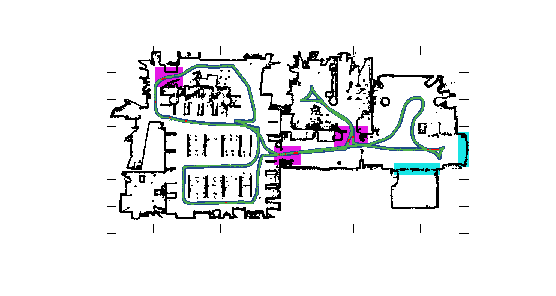
\includegraphics[trim={0 0 0 0.4cm},clip]{./figures/experiments/a/trajectory}}%
    \gplfronttext
  \end{picture}%
\endgroup

  \vspace{-0.7cm}
  \caption{\small The map of the CSAL environment (black), the trajectory of
           the sensor (blue), and CBGL's estimated positions of the sensor
           (green). Sensor poses for which CBGL's output exhibits position error
           larger than $\delta_{\bm{l}} = 0.5$ m are marked with red, sources
           of great range noise with cyan, and regions around doors with
           purple. A total of $N_S = 6669$ pose estimations take place.
           Estimation is performed for each sensor pose independently of
           previous estimates and measurements}
  \vspace{-0.5cm}
  \label{fig:a:map_and_trajectory}
\end{figure}

\begin{figure}
  \vspace{-0.4cm}
  \definecolor{g1}{RGB}{200 200 200}
\definecolor{g2}{RGB}{162 162 162}
\definecolor{g3}{RGB}{137 137 137}
\definecolor{g4}{RGB}{77 175 74}

% GNUPLOT: LaTeX picture with Postscript
\begingroup
  \makeatletter
  \providecommand\color[2][]{%
    \GenericError{(gnuplot) \space\space\space\@spaces}{%
      Package color not loaded in conjunction with
      terminal option `colourtext'%
    }{See the gnuplot documentation for explanation.%
    }{Either use 'blacktext' in gnuplot or load the package
      color.sty in LaTeX.}%
    \renewcommand\color[2][]{}%
  }%
  \providecommand\includegraphics[2][]{%
    \GenericError{(gnuplot) \space\space\space\@spaces}{%
      Package graphicx or graphics not loaded%
    }{See the gnuplot documentation for explanation.%
    }{The gnuplot epslatex terminal needs graphicx.sty or graphics.sty.}%
    \renewcommand\includegraphics[2][]{}%
  }%
  \providecommand\rotatebox[2]{#2}%
  \@ifundefined{ifGPcolor}{%
    \newif\ifGPcolor
    \GPcolorfalse
  }{}%
  \@ifundefined{ifGPblacktext}{%
    \newif\ifGPblacktext
    \GPblacktexttrue
  }{}%
  % define a \g@addto@macro without @ in the name:
  \let\gplgaddtomacro\g@addto@macro
  % define empty templates for all commands taking text:
  \gdef\gplfronttext{}%
  \gdef\gplfronttext{}%
  \makeatother
  \ifGPblacktext
    % no textcolor at all
    \def\colorrgb#1{}%
    \def\colorgray#1{}%
  \else
    % gray or color?
    \ifGPcolor
      \def\colorrgb#1{\color[rgb]{#1}}%
      \def\colorgray#1{\color[gray]{#1}}%
      \expandafter\def\csname LTw\endcsname{\color{white}}%
      \expandafter\def\csname LTb\endcsname{\color{black}}%
      \expandafter\def\csname LTa\endcsname{\color{black}}%
      \expandafter\def\csname LT0\endcsname{\color[rgb]{1,0,0}}%
      \expandafter\def\csname LT1\endcsname{\color[rgb]{0,1,0}}%
      \expandafter\def\csname LT2\endcsname{\color[rgb]{0,0,1}}%
      \expandafter\def\csname LT3\endcsname{\color[rgb]{1,0,1}}%
      \expandafter\def\csname LT4\endcsname{\color[rgb]{0,1,1}}%
      \expandafter\def\csname LT5\endcsname{\color[rgb]{1,1,0}}%
      \expandafter\def\csname LT6\endcsname{\color[rgb]{0,0,0}}%
      \expandafter\def\csname LT7\endcsname{\color[rgb]{1,0.3,0}}%
      \expandafter\def\csname LT8\endcsname{\color[rgb]{0.5,0.5,0.5}}%
    \else
      % gray
      \def\colorrgb#1{\color{black}}%
      \def\colorgray#1{\color[gray]{#1}}%
      \expandafter\def\csname LTw\endcsname{\color{white}}%
      \expandafter\def\csname LTb\endcsname{\color{black}}%
      \expandafter\def\csname LTa\endcsname{\color{black}}%
      \expandafter\def\csname LT0\endcsname{\color{black}}%
      \expandafter\def\csname LT1\endcsname{\color{black}}%
      \expandafter\def\csname LT2\endcsname{\color{black}}%
      \expandafter\def\csname LT3\endcsname{\color{black}}%
      \expandafter\def\csname LT4\endcsname{\color{black}}%
      \expandafter\def\csname LT5\endcsname{\color{black}}%
      \expandafter\def\csname LT6\endcsname{\color{black}}%
      \expandafter\def\csname LT7\endcsname{\color{black}}%
      \expandafter\def\csname LT8\endcsname{\color{black}}%
    \fi
  \fi
    \setlength{\unitlength}{0.0500bp}%
    \ifx\gptboxheight\undefined%
      \newlength{\gptboxheight}%
      \newlength{\gptboxwidth}%
      \newsavebox{\gptboxtext}%
    \fi%
    \setlength{\fboxrule}{0.5pt}%
    \setlength{\fboxsep}{1pt}%
\begin{picture}(5000.00,2500.00)%
    \gplgaddtomacro\gplfronttext{%
      \colorrgb{0.15,0.15,0.15}%
      \put(1000,2600){\makebox(0,0){\strut{}{\color{g4}{\rule[0.6mm]{0.5cm}{0.5mm}}} \footnotesize Output}}
      \put(2500,2600){\makebox(0,0){\strut{}{\color{g3}{\rule[0.6mm]{0.5cm}{0.5mm}}} \footnotesize $\mathcal{H}_1[\arg \min f_{\psi}^{\bm{M}}(\mathcal{H}_2)]$}}
      \put(3900,2600){\makebox(0,0){\strut{}{\color{g2}{\rule[0.6mm]{0.5cm}{0.5mm}}} \footnotesize $\mathcal{H}_1$}}
      \put(4500,2600){\makebox(0,0){\strut{}{\color{g1}{\rule[0.6mm]{0.5cm}{0.5mm}}} \footnotesize $\mathcal{H}$}}
      \put(468,250){\makebox(0,0)[r]{\strut{}\footnotesize $0.0$}}%
      \colorrgb{0.15,0.15,0.15}%
      \put(468,750){\makebox(0,0)[r]{\strut{}\footnotesize $0.25$}}%
      \colorrgb{0.15,0.15,0.15}%
      \put(468,1250){\makebox(0,0)[r]{\strut{}\footnotesize $0.50$}}%
      \colorrgb{0.15,0.15,0.15}%
      \put(468,1793){\makebox(0,0)[r]{\strut{}\footnotesize $0.772$}}%
      \colorrgb{0.15,0.15,0.15}%
      \put(468,2105){\makebox(0,0)[r]{\strut{}\footnotesize $0.928$}}%
      \colorrgb{0.15,0.15,0.15}%
      \put(468,2231){\makebox(0,0)[r]{\strut{}\footnotesize $0.991$}}%
      \colorrgb{0.15,0.15,0.15}%
      \put(500,30){\makebox(0,0){\strut{}\footnotesize $5$\texttt{e}-$05$}}%
      \colorrgb{0.15,0.15,0.15}%
      \put(970,30){\makebox(0,0){\strut{}\footnotesize $0.01$}}%
      \colorrgb{0.15,0.15,0.15}%
      \put(1576,30){\makebox(0,0){\strut{}\footnotesize $0.50$}}%
      \colorrgb{0.15,0.15,0.15}%
      %\put(2040,30){\makebox(0,0){\strut{}\footnotesize $10.0$}}%
      \colorrgb{0.15,0.15,0.15}%
      \put(2199,30){\makebox(0,0){\strut{}\footnotesize $27.86$}}%
    }%
    \gplgaddtomacro\gplfronttext{%
      \colorrgb{0.15,0.15,0.15}%
      \put(1349,-300){\makebox(0,0){\strut{}\footnotesize Outliers locational threshold $\delta_{\bm{l}}$ [m]}}%
    }%
    \gplgaddtomacro\gplfronttext{%
      \colorrgb{0.15,0.15,0.15}%
      \put(2893,250){\makebox(0,0)[r]{\strut{}\footnotesize $0.0$}}%
      \colorrgb{0.15,0.15,0.15}%
      \put(2893,750){\makebox(0,0)[r]{\strut{}\footnotesize $0.25$}}%
      \colorrgb{0.15,0.15,0.15}%
      \put(2893,999){\makebox(0,0)[r]{\strut{}\footnotesize $0.375$}}%
      \colorrgb{0.15,0.15,0.15}%
      \put(2893,1153){\makebox(0,0)[r]{\strut{}\footnotesize $0.452$}}%
      \colorrgb{0.15,0.15,0.15}%
      \put(2893,2137){\makebox(0,0)[r]{\strut{}\footnotesize $0.944$}}%
      \colorrgb{0.15,0.15,0.15}%
      \put(2925,30){\makebox(0,0){\strut{}\footnotesize $4$\texttt{e}-$05$}}%
      \colorrgb{0.15,0.15,0.15}%
      \put(3740,30){\makebox(0,0){\strut{}\footnotesize $\frac{\pi}{1000}$}}%
      \colorrgb{0.15,0.15,0.15}%
      \put(4114,30){\makebox(0,0){\strut{}\footnotesize $\frac{\pi}{100}$}}%
      \colorrgb{0.15,0.15,0.15}%
      \put(4749,30){\makebox(0,0){\strut{}\footnotesize $\pi$}}%
    }%
    \gplgaddtomacro\gplfronttext{%
      \colorrgb{0.15,0.15,0.15}%
      \put(3837,-300){\makebox(0,0){\strut{}\footnotesize Outliers angular threshold $\delta_{\alpha}$ [rad]}}%
    }%
    \put(0,0){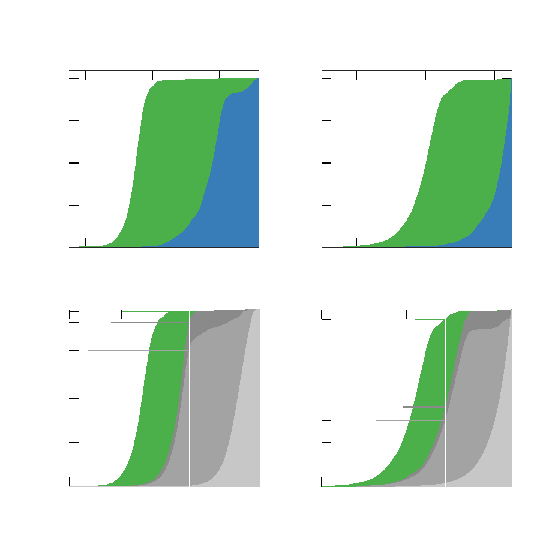
\includegraphics{./figures/experiments/a/awesomeness}}%
    \gplfronttext
  \end{picture}%
\endgroup

  \vspace{0.01cm}
  \caption{\small Proportions of pose estimates whose position and orientation
           error is lower than corresponding thresholds $\delta_{\bm{l}}$ and
           $\delta_{\theta}$. Top: ALS vs CBGL. Bottom: CBGL and internal pose
           estimate sets.  Approximately $77\%$ of all bottom-$k$ pose
           estimates---the contents of $\mathcal{H}_1$ sets, populated via rank
           fields as described in sections \ref{section:definitions} and
           \ref{section:the_proposed_method}---exhibit position errors lower
           than $\delta_{\bm{l}} = 0.5$ m for $k=10$, and so do over $99\%$ of
           CBGL's final pose estimates. The improvement in position and
           orientation induced by scan--to--map-scan matching is captured by
           the difference between the output (i.e.  $\mathcal{H}_2[\arg \min
           f_{\psi}^{\bm{M}}(\mathcal{H}_2)]$) and $\mathcal{H}_1[\arg \min
           f_{\psi}^{\bm{M}}(\mathcal{H}_2)]$}
  \vspace{-0.5cm}
  \label{fig:a:awesomeness}
\end{figure}


%%%%%%%%%%%%%%%%%%%%%%%%%%%%%%%%%%%%%%%%%%%%%%%%%%%%%%%%%%%%%%%%%%%%%%%%%%%%%%%%
\subsection{Simulations against sources of uncertainty}
\label{subsec:exp_b}

The second type of test concerns the main limiting factor of global
localisation methods, i.e. uncertainty---:arising e.g. from spurious
measurements, repeatability of surroundings, missing range information, or
their combinations. For this reason the experimental procedure of
\cite{Filotheou2022g} is extended here for the two methods tested therein,
i.e. PGL-FMIC and PGL-PLICP, and then for CBGL, ALS, MCL \cite{mcl}, and GMCL
\cite{gmcl}.  Specifically these methods are tested against the two most
challenging environments, i.e. WAREHOUSE and WILLOWGARAGE, in which a panoramic
range sensor is placed at $16$ different poses for $N = 100$ independent
attempts at global localisation per tested method. The tests are conducted with
the use of a sensor whose number of rays $N_s = 360$, maximum range
$r_{\max} = 10.0$ m, and noise $\mathcal{N}(0, 0.05^2)$ [m,m$^2$]. CBGL's
internal \texttt{sm2} method is chosen to be \texttt{x1}
\cite{Filotheou2023a} due to the periodicity of the range signal,
\texttt{x1}'s improved results over \texttt{sm2} matching state of the
art methods, and its ability in matching scans captured from greater initial
locational distances than ICP alternatives. The latter translates to the need
for smaller initial hypothesis sets: for each environment the locational
density is set to $3$\texttt{e}+04 divided by the free space area
of each environment. For Monte Carlo approaches MCL and GMCL the number of
initial hypotheses is also set to $3$\texttt{e}+04.

The maximum range of the sensor is such that the geometry of environment
WAREHOUSE causes (disorderly) extended lack of sampling of the sensor's
surrounding environment, which limits available information and may therefore
produce spurious measurements and increase ambiguities between candidate
estimates. In WILLOWGARAGE on the other hand, almost all sensor placements
result in complete sampling of its surroundings, but the sensor is purposefully
posed in such conditions as to challenge the localisation methods' ability to
perform fine distinctions between similar surroundings. Figure
\ref{fig:b:inliers_per_pose} depicts the percentage of outputs whose position
error is lower than $\delta_{\bm{l}} = 0.5$ m per tested pose, and figure
\ref{fig:b:execution_times} depicts the overall distribution of execution times
per tested environment and algorithm. CBGL's mean execution time in environment
WAREHOUSE is $\mu_t^W = 7.98$ sec and in WILLOWGARAGE $\mu_t^{G} = 3.59$ sec.
Although the cardinality of set $\mathcal{H}$ is equal for both environments
CBGL's execution times are uneven due to \texttt{x1}'s increased execution
time when dealing with scans with missing range information. Notwithstanding
the aforementioned sources of uncertainty, CBGL manages to exhibit the highest
number of inliers in each environment tested.


\begin{figure}
  \definecolor{c1}{RGB}{228,26,28}
\definecolor{c2}{RGB}{55,126,184}
\definecolor{c3}{RGB}{255,0,255}
\definecolor{c4}{RGB}{152,78,163}
\definecolor{c5}{RGB}{255,127,0}
\definecolor{c6}{RGB}{77,175,74}
\hspace{0.5cm}

% GNUPLOT: LaTeX picture with Postscript
\begingroup
  \makeatletter
  \providecommand\color[2][]{%
    \GenericError{(gnuplot) \space\space\space\@spaces}{%
      Package color not loaded in conjunction with
      terminal option `colourtext'%
    }{See the gnuplot documentation for explanation.%
    }{Either use 'blacktext' in gnuplot or load the package
      color.sty in LaTeX.}%
    \renewcommand\color[2][]{}%
  }%
  \providecommand\includegraphics[2][]{%
    \GenericError{(gnuplot) \space\space\space\@spaces}{%
      Package graphicx or graphics not loaded%
    }{See the gnuplot documentation for explanation.%
    }{The gnuplot epslatex terminal needs graphicx.sty or graphics.sty.}%
    \renewcommand\includegraphics[2][]{}%
  }%
  \providecommand\rotatebox[2]{#2}%
  \@ifundefined{ifGPcolor}{%
    \newif\ifGPcolor
    \GPcolorfalse
  }{}%
  \@ifundefined{ifGPblacktext}{%
    \newif\ifGPblacktext
    \GPblacktexttrue
  }{}%
  % define a \g@addto@macro without @ in the name:
  \let\gplgaddtomacro\g@addto@macro
  % define empty templates for all commands taking text:
  \gdef\gplfronttext{}%
  \gdef\gplfronttext{}%
  \makeatother
  \ifGPblacktext
    % no textcolor at all
    \def\colorrgb#1{}%
    \def\colorgray#1{}%
  \else
    % gray or color?
    \ifGPcolor
      \def\colorrgb#1{\color[rgb]{#1}}%
      \def\colorgray#1{\color[gray]{#1}}%
      \expandafter\def\csname LTw\endcsname{\color{white}}%
      \expandafter\def\csname LTb\endcsname{\color{black}}%
      \expandafter\def\csname LTa\endcsname{\color{black}}%
      \expandafter\def\csname LT0\endcsname{\color[rgb]{1,0,0}}%
      \expandafter\def\csname LT1\endcsname{\color[rgb]{0,1,0}}%
      \expandafter\def\csname LT2\endcsname{\color[rgb]{0,0,1}}%
      \expandafter\def\csname LT3\endcsname{\color[rgb]{1,0,1}}%
      \expandafter\def\csname LT4\endcsname{\color[rgb]{0,1,1}}%
      \expandafter\def\csname LT5\endcsname{\color[rgb]{1,1,0}}%
      \expandafter\def\csname LT6\endcsname{\color[rgb]{0,0,0}}%
      \expandafter\def\csname LT7\endcsname{\color[rgb]{1,0.3,0}}%
      \expandafter\def\csname LT8\endcsname{\color[rgb]{0.5,0.5,0.5}}%
    \else
      % gray
      \def\colorrgb#1{\color{black}}%
      \def\colorgray#1{\color[gray]{#1}}%
      \expandafter\def\csname LTw\endcsname{\color{white}}%
      \expandafter\def\csname LTb\endcsname{\color{black}}%
      \expandafter\def\csname LTa\endcsname{\color{black}}%
      \expandafter\def\csname LT0\endcsname{\color{black}}%
      \expandafter\def\csname LT1\endcsname{\color{black}}%
      \expandafter\def\csname LT2\endcsname{\color{black}}%
      \expandafter\def\csname LT3\endcsname{\color{black}}%
      \expandafter\def\csname LT4\endcsname{\color{black}}%
      \expandafter\def\csname LT5\endcsname{\color{black}}%
      \expandafter\def\csname LT6\endcsname{\color{black}}%
      \expandafter\def\csname LT7\endcsname{\color{black}}%
      \expandafter\def\csname LT8\endcsname{\color{black}}%
    \fi
  \fi
    \setlength{\unitlength}{0.0500bp}%
    \ifx\gptboxheight\undefined%
      \newlength{\gptboxheight}%
      \newlength{\gptboxwidth}%
      \newsavebox{\gptboxtext}%
    \fi%
    \setlength{\fboxrule}{0.5pt}%
    \setlength{\fboxsep}{1pt}%
  \hspace{0.5cm}
\begin{picture}(5000.00,3000.00)%
    \gplgaddtomacro\gplfronttext{%
      \colorrgb{0.15,0.15,0.15}%
      \put(368,1724){\makebox(0,0)[r]{\strut{}\footnotesize $0\%$}}%
      \colorrgb{0.15,0.15,0.15}%
      \put(368,1968){\makebox(0,0)[r]{\strut{}\footnotesize $25\%$}}%
      \colorrgb{0.15,0.15,0.15}%
      \put(368,2212){\makebox(0,0)[r]{\strut{}\footnotesize $50\%$}}%
      \colorrgb{0.15,0.15,0.15}%
      \put(368,2455){\makebox(0,0)[r]{\strut{}\footnotesize $75\%$}}%
      \colorrgb{0.15,0.15,0.15}%
      \put(368,2699){\makebox(0,0)[r]{\strut{}\footnotesize $100\%$}}%
      \colorrgb{0.15,0.15,0.15}%
      \put(833,1504){\makebox(0,0){\strut{}\footnotesize $\bm{p}_a^W$}}%
      \colorrgb{0.15,0.15,0.15}%
      \put(1500,1504){\makebox(0,0){\strut{}\footnotesize $\bm{p}_b^W$}}%
      \colorrgb{0.15,0.15,0.15}%
      \put(2166,1504){\makebox(0,0){\strut{}\footnotesize $\bm{p}_c^W$}}%
      \colorrgb{0.15,0.15,0.15}%
      \put(2833,1504){\makebox(0,0){\strut{}\footnotesize $\bm{p}_d^W$}}%
      \colorrgb{0.15,0.15,0.15}%
      \put(3499,1504){\makebox(0,0){\strut{}\footnotesize $\bm{p}_f^W$}}%
      \colorrgb{0.15,0.15,0.15}%
      \put(4166,1504){\makebox(0,0){\strut{}\footnotesize $\bm{p}_g^W$}}%
    }%
    \gplgaddtomacro\gplfronttext{%
      \colorrgb{0.15,0.15,0.15}%
      \put(-198,2211){\rotatebox{90}{\makebox(0,0){\strut{}\footnotesize WAREHOUSE}}}%
      \put( 200,3000){\makebox(0,0){\strut{}{\color{c1}{\rule[0.6mm]{0.3cm}{0.5mm}}} \scriptsize MCL}}
      \put( 800,3000){\makebox(0,0){\strut{}{\color{c2}{\rule[0.6mm]{0.3cm}{0.5mm}}} \scriptsize ALS}}
      \put(1450,3000){\makebox(0,0){\strut{}{\color{c3}{\rule[0.6mm]{0.3cm}{0.5mm}}} \scriptsize GMCL}}
      \put(2300,3000){\makebox(0,0){\strut{}{\color{c4}{\rule[0.6mm]{0.3cm}{0.5mm}}} \scriptsize PGL-FMIC}}
      \put(3300,3000){\makebox(0,0){\strut{}{\color{c5}{\rule[0.6mm]{0.3cm}{0.5mm}}} \scriptsize PGL-PLICP}}
      \put(4250,3000){\makebox(0,0){\strut{}{\color{c6}{\rule[0.6mm]{0.3cm}{0.5mm}}} \scriptsize CBGL}}
    }%
    \gplgaddtomacro\gplfronttext{%
      \colorrgb{0.15,0.15,0.15}%
      \put(368,300){\makebox(0,0)[r]{\strut{}\footnotesize $0\%$}}%
      \colorrgb{0.15,0.15,0.15}%
      \put(368,544){\makebox(0,0)[r]{\strut{}\footnotesize $25\%$}}%
      \colorrgb{0.15,0.15,0.15}%
      \put(368,787){\makebox(0,0)[r]{\strut{}\footnotesize $50\%$}}%
      \colorrgb{0.15,0.15,0.15}%
      \put(368,1031){\makebox(0,0)[r]{\strut{}\footnotesize $75\%$}}%
      \colorrgb{0.15,0.15,0.15}%
      \put(368,1274){\makebox(0,0)[r]{\strut{}\footnotesize $100\%$}}%
      \colorrgb{0.15,0.15,0.15}%
      \put(700,80){\makebox(0,0){\strut{}\footnotesize $\bm{p}_a^G$}}%
      \colorrgb{0.15,0.15,0.15}%
      \put(1100,80){\makebox(0,0){\strut{}\footnotesize $\bm{p}_b^G$}}%
      \colorrgb{0.15,0.15,0.15}%
      \put(1500,80){\makebox(0,0){\strut{}\footnotesize $\bm{p}_c^G$}}%
      \colorrgb{0.15,0.15,0.15}%
      \put(1900,80){\makebox(0,0){\strut{}\footnotesize $\bm{p}_d^G$}}%
      \colorrgb{0.15,0.15,0.15}%
      \put(2300,80){\makebox(0,0){\strut{}\footnotesize $\bm{p}_e^G$}}%
      \colorrgb{0.15,0.15,0.15}%
      \put(2699,80){\makebox(0,0){\strut{}\footnotesize $\bm{p}_f^G$}}%
      \colorrgb{0.15,0.15,0.15}%
      \put(3099,80){\makebox(0,0){\strut{}\footnotesize $\bm{p}_g^G$}}%
      \colorrgb{0.15,0.15,0.15}%
      \put(3499,80){\makebox(0,0){\strut{}\footnotesize $\bm{p}_h^G$}}%
      \colorrgb{0.15,0.15,0.15}%
      \put(3899,80){\makebox(0,0){\strut{}\footnotesize $\bm{p}_i^G$}}%
      \colorrgb{0.15,0.15,0.15}%
      \put(4299,80){\makebox(0,0){\strut{}\footnotesize $\bm{p}_j^G$}}%
    }%
    \gplgaddtomacro\gplfronttext{%
      \colorrgb{0.15,0.15,0.15}%
      \put(-198,787){\rotatebox{90}{\makebox(0,0){\strut{}\footnotesize WILLOWGARAGE}}}%
    }%
    \put(0,0){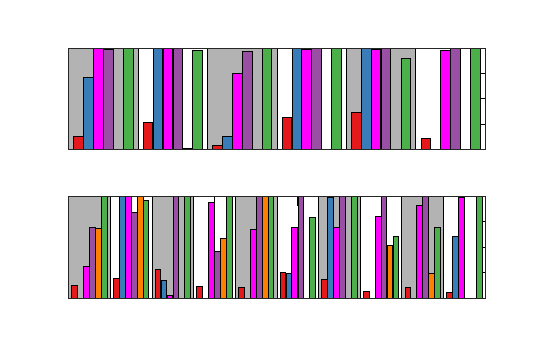
\includegraphics{./figures/experiments/b/inliers_per_pose}}%
    \gplfronttext
  \end{picture}%
\endgroup

  \caption{\small Percent proportions of pose outputs whose position error is
           lower than $\delta_{\bm{l}} = 0.5$ m per tested environment, pose,
           and method. Overall CBGL (green) features the highest number of
           inlier poses}
  \label{fig:b:inliers_per_pose}
\end{figure}

\begin{figure}
  \definecolor{c1}{RGB}{228,26,28}
\definecolor{c2}{RGB}{55,126,184}
\definecolor{c3}{RGB}{255,0,255}
\definecolor{c4}{RGB}{152,78,163}
\definecolor{c5}{RGB}{255,127,0}
\definecolor{c6}{RGB}{77,175,74}

% GNUPLOT: LaTeX picture with Postscript
\begingroup
  \makeatletter
  \providecommand\color[2][]{%
    \GenericError{(gnuplot) \space\space\space\@spaces}{%
      Package color not loaded in conjunction with
      terminal option `colourtext'%
    }{See the gnuplot documentation for explanation.%
    }{Either use 'blacktext' in gnuplot or load the package
      color.sty in LaTeX.}%
    \renewcommand\color[2][]{}%
  }%
  \providecommand\includegraphics[2][]{%
    \GenericError{(gnuplot) \space\space\space\@spaces}{%
      Package graphicx or graphics not loaded%
    }{See the gnuplot documentation for explanation.%
    }{The gnuplot epslatex terminal needs graphicx.sty or graphics.sty.}%
    \renewcommand\includegraphics[2][]{}%
  }%
  \providecommand\rotatebox[2]{#2}%
  \@ifundefined{ifGPcolor}{%
    \newif\ifGPcolor
    \GPcolorfalse
  }{}%
  \@ifundefined{ifGPblacktext}{%
    \newif\ifGPblacktext
    \GPblacktexttrue
  }{}%
  % define a \g@addto@macro without @ in the name:
  \let\gplgaddtomacro\g@addto@macro
  % define empty templates for all commands taking text:
  \gdef\gplfronttext{}%
  \gdef\gplfronttext{}%
  \makeatother
  \ifGPblacktext
    % no textcolor at all
    \def\colorrgb#1{}%
    \def\colorgray#1{}%
  \else
    % gray or color?
    \ifGPcolor
      \def\colorrgb#1{\color[rgb]{#1}}%
      \def\colorgray#1{\color[gray]{#1}}%
      \expandafter\def\csname LTw\endcsname{\color{white}}%
      \expandafter\def\csname LTb\endcsname{\color{black}}%
      \expandafter\def\csname LTa\endcsname{\color{black}}%
      \expandafter\def\csname LT0\endcsname{\color[rgb]{1,0,0}}%
      \expandafter\def\csname LT1\endcsname{\color[rgb]{0,1,0}}%
      \expandafter\def\csname LT2\endcsname{\color[rgb]{0,0,1}}%
      \expandafter\def\csname LT3\endcsname{\color[rgb]{1,0,1}}%
      \expandafter\def\csname LT4\endcsname{\color[rgb]{0,1,1}}%
      \expandafter\def\csname LT5\endcsname{\color[rgb]{1,1,0}}%
      \expandafter\def\csname LT6\endcsname{\color[rgb]{0,0,0}}%
      \expandafter\def\csname LT7\endcsname{\color[rgb]{1,0.3,0}}%
      \expandafter\def\csname LT8\endcsname{\color[rgb]{0.5,0.5,0.5}}%
    \else
      % gray
      \def\colorrgb#1{\color{black}}%
      \def\colorgray#1{\color[gray]{#1}}%
      \expandafter\def\csname LTw\endcsname{\color{white}}%
      \expandafter\def\csname LTb\endcsname{\color{black}}%
      \expandafter\def\csname LTa\endcsname{\color{black}}%
      \expandafter\def\csname LT0\endcsname{\color{black}}%
      \expandafter\def\csname LT1\endcsname{\color{black}}%
      \expandafter\def\csname LT2\endcsname{\color{black}}%
      \expandafter\def\csname LT3\endcsname{\color{black}}%
      \expandafter\def\csname LT4\endcsname{\color{black}}%
      \expandafter\def\csname LT5\endcsname{\color{black}}%
      \expandafter\def\csname LT6\endcsname{\color{black}}%
      \expandafter\def\csname LT7\endcsname{\color{black}}%
      \expandafter\def\csname LT8\endcsname{\color{black}}%
    \fi
  \fi
    \setlength{\unitlength}{0.0500bp}%
    \ifx\gptboxheight\undefined%
      \newlength{\gptboxheight}%
      \newlength{\gptboxwidth}%
      \newsavebox{\gptboxtext}%
    \fi%
    \setlength{\fboxrule}{0.5pt}%
    \setlength{\fboxsep}{1pt}%
\begin{picture}(5000.00,1500.00)%
    \gplgaddtomacro\gplfronttext{%
      \colorrgb{0.15,0.15,0.15}%
      \put(368,267){\makebox(0,0)[r]{\strut{}\footnotesize $10^{0}$}}%
      \colorrgb{0.15,0.15,0.15}%
      \put(368,657){\makebox(0,0)[r]{\strut{}\footnotesize $10^{1}$}}%
      \colorrgb{0.15,0.15,0.15}%
      \put(368,1046){\makebox(0,0)[r]{\strut{}\footnotesize $10^{2}$}}%
    }%
    \gplgaddtomacro\gplfronttext{%
      \colorrgb{0.15,0.15,0.15}%
      \put(1474,-70){\makebox(0,0){\strut{}\footnotesize WAREHOUSE}}%
      \put( 400,1500){\makebox(0,0){\strut{}{\color{c1}{\rule[0.6mm]{0.3cm}{0.5mm}}} \scriptsize MCL}}
      \put(1000,1500){\makebox(0,0){\strut{}{\color{c2}{\rule[0.6mm]{0.3cm}{0.5mm}}} \scriptsize ALS}}
      \put(1650,1500){\makebox(0,0){\strut{}{\color{c3}{\rule[0.6mm]{0.3cm}{0.5mm}}} \scriptsize GMCL}}
      \put(2500,1500){\makebox(0,0){\strut{}{\color{c4}{\rule[0.6mm]{0.3cm}{0.5mm}}} \scriptsize PGL-FMIC}}
      \put(3500,1500){\makebox(0,0){\strut{}{\color{c5}{\rule[0.6mm]{0.3cm}{0.5mm}}} \scriptsize PGL-PLICP}}
      \put(4450,1500){\makebox(0,0){\strut{}{\color{c6}{\rule[0.6mm]{0.3cm}{0.5mm}}} \scriptsize CBGL}}
    }%
    \gplgaddtomacro\gplfronttext{%
      \colorrgb{0.15,0.15,0.15}%
      \put(2418,267){\makebox(0,0)[r]{\strut{}\footnotesize $10^{0}$}}%
      \colorrgb{0.15,0.15,0.15}%
      \put(2418,657){\makebox(0,0)[r]{\strut{}\footnotesize $10^{1}$}}%
      \colorrgb{0.15,0.15,0.15}%
      \put(2418,1046){\makebox(0,0)[r]{\strut{}\footnotesize $10^{2}$}}%
    }%
    \gplgaddtomacro\gplfronttext{%
      \colorrgb{0.15,0.15,0.15}%
      \put(3524,-70){\makebox(0,0){\strut{}\footnotesize WILLOWGARAGE}}%
    }%
    \put(0,0){\includegraphics{./figures/experiments/b/exec_times}}%
    \gplfronttext
  \end{picture}%
\endgroup

  \vspace{0.1cm}
  \caption{\small Distribution of execution times per tested environment and
           algorithm in seconds for $N_s = 360$ rays. CBGL's execution time is
           at least eighteen times lower than other Monte Carlo approaches in
           WILLOWGARAGE and four times lower in WAREHOUSE}
  \label{fig:b:execution_times}
  \vspace{-0.5cm}
\end{figure}


%%%%%%%%%%%%%%%%%%%%%%%%%%%%%%%%%%%%%%%%%%%%%%%%%%%%%%%%%%%%%%%%%%%%%%%%%%%%%%%%
\subsection{Simulations against environmental and \texttt{sm2} algorithmic disparity }
\label{subsec:exp_c}

The third type of test aims to inquire how the performance of CBGL scales with
respect to increasing environment area (and therefore to increased number of
hypotheses), environment diversity, sensor angular range, and choice of
overlying \texttt{sm2} method. CBGL is tested once in each of
$N_E \simeq 4.5$\texttt{e}+$04$ environments, generated via the experimental
procedure of \cite{Filotheou2023a}, which utilises five established and
publicly available benchmark datasets provided courtesy of the Department of
Computer Science, University of Freiburg \cite{datasets_link}.  The coordinates
of every map corresponding to each environment are corrupted by noise
$\mathcal{N}(0,0.05^2)$ [m, m$^2$]. The angular range of the range sensor
varies according to the overlying scan--to--map-scan matching method used: for
NDT \cite{ndt}, FastGICP \cite{fgi}, and FastVGICP \cite{fvg}: $\lambda =
3\pi/2$ rad; for \texttt{x1}: $\lambda = 2\pi$ rad. Measurement noise is
$\mathcal{N}(0,0.03^2)$ [m,m$^2$]. As in subsection \ref{subsec:exp_a} the
choice of field densities and $k$ is $(d_{\bm{l}},d_{\alpha},k) = (40, 2^5,
10)$.

Figure \ref{fig:c:errors_and_time} illustrates that, with the exception of
NDT, all versions of CBGL exhibit mean positional errors less than $1.0$ m; its
combination with \texttt{x1} exhibits a mean error of approximately $0.5$ m.
The evidence support the claim that CBGL is robust to sensor angular range,
as the distributions of errors are indistinguishable between bottom-$k$
($\mathcal{H}_1$) sets for $k=10$.

Figure \ref{fig:c:time_analysis} shows the execution time of FastVGICP and
\texttt{x1} as a function of environmental area, and \texttt{x1}'s timing
breakdown with respect to (a) calculating up to line \ref{alg:cbgl:h1} of
Algorithm \ref{alg:cbgl} (that is CBGL's total time minus scan--to--map-scan
matching time) and (b) computing map-scans, as proportions of total execution
time. Given the evidence one may conclude that CBGL's execution time is linear
with respect to environment area for areas larger than 200 m$^2$, with slope
$l = 17$\texttt{e}-$03$.

\begin{figure}
  \definecolor{c0}{RGB}{162 162 162}
\definecolor{c1}{RGB}{102 194 165}
\definecolor{c2}{RGB}{252 141 98}
\definecolor{c3}{RGB}{41 160 203}
\definecolor{c4}{RGB}{231 138 195}

% GNUPLOT: LaTeX picture with Postscript
\begingroup
  \makeatletter
  \providecommand\color[2][]{%
    \GenericError{(gnuplot) \space\space\space\@spaces}{%
      Package color not loaded in conjunction with
      terminal option `colourtext'%
    }{See the gnuplot documentation for explanation.%
    }{Either use 'blacktext' in gnuplot or load the package
      color.sty in LaTeX.}%
    \renewcommand\color[2][]{}%
  }%
  \providecommand\includegraphics[2][]{%
    \GenericError{(gnuplot) \space\space\space\@spaces}{%
      Package graphicx or graphics not loaded%
    }{See the gnuplot documentation for explanation.%
    }{The gnuplot epslatex terminal needs graphicx.sty or graphics.sty.}%
    \renewcommand\includegraphics[2][]{}%
  }%
  \providecommand\rotatebox[2]{#2}%
  \@ifundefined{ifGPcolor}{%
    \newif\ifGPcolor
    \GPcolorfalse
  }{}%
  \@ifundefined{ifGPblacktext}{%
    \newif\ifGPblacktext
    \GPblacktexttrue
  }{}%
  % define a \g@addto@macro without @ in the name:
  \let\gplgaddtomacro\g@addto@macro
  % define empty templates for all commands taking text:
  \gdef\gplfronttext{}%
  \gdef\gplfronttext{}%
  \makeatother
  \ifGPblacktext
    % no textcolor at all
    \def\colorrgb#1{}%
    \def\colorgray#1{}%
  \else
    % gray or color?
    \ifGPcolor
      \def\colorrgb#1{\color[rgb]{#1}}%
      \def\colorgray#1{\color[gray]{#1}}%
      \expandafter\def\csname LTw\endcsname{\color{white}}%
      \expandafter\def\csname LTb\endcsname{\color{black}}%
      \expandafter\def\csname LTa\endcsname{\color{black}}%
      \expandafter\def\csname LT0\endcsname{\color[rgb]{1,0,0}}%
      \expandafter\def\csname LT1\endcsname{\color[rgb]{0,1,0}}%
      \expandafter\def\csname LT2\endcsname{\color[rgb]{0,0,1}}%
      \expandafter\def\csname LT3\endcsname{\color[rgb]{1,0,1}}%
      \expandafter\def\csname LT4\endcsname{\color[rgb]{0,1,1}}%
      \expandafter\def\csname LT5\endcsname{\color[rgb]{1,1,0}}%
      \expandafter\def\csname LT6\endcsname{\color[rgb]{0,0,0}}%
      \expandafter\def\csname LT7\endcsname{\color[rgb]{1,0.3,0}}%
      \expandafter\def\csname LT8\endcsname{\color[rgb]{0.5,0.5,0.5}}%
    \else
      % gray
      \def\colorrgb#1{\color{black}}%
      \def\colorgray#1{\color[gray]{#1}}%
      \expandafter\def\csname LTw\endcsname{\color{white}}%
      \expandafter\def\csname LTb\endcsname{\color{black}}%
      \expandafter\def\csname LTa\endcsname{\color{black}}%
      \expandafter\def\csname LT0\endcsname{\color{black}}%
      \expandafter\def\csname LT1\endcsname{\color{black}}%
      \expandafter\def\csname LT2\endcsname{\color{black}}%
      \expandafter\def\csname LT3\endcsname{\color{black}}%
      \expandafter\def\csname LT4\endcsname{\color{black}}%
      \expandafter\def\csname LT5\endcsname{\color{black}}%
      \expandafter\def\csname LT6\endcsname{\color{black}}%
      \expandafter\def\csname LT7\endcsname{\color{black}}%
      \expandafter\def\csname LT8\endcsname{\color{black}}%
    \fi
  \fi
    \setlength{\unitlength}{0.0500bp}%
    \ifx\gptboxheight\undefined%
      \newlength{\gptboxheight}%
      \newlength{\gptboxwidth}%
      \newsavebox{\gptboxtext}%
    \fi%
    \setlength{\fboxrule}{0.5pt}%
    \setlength{\fboxsep}{1pt}%
\begin{picture}(5000.00,1500.00)%
    \gplgaddtomacro\gplfronttext{%
      \colorrgb{0.15,0.15,0.15}%
      \put(468,224){\makebox(0,0)[r]{\strut{}\scriptsize $10^{-4}$}}%
      \colorrgb{0.15,0.15,0.15}%
      \put(468,468){\makebox(0,0)[r]{\strut{}\scriptsize $10^{-3}$}}%
      \colorrgb{0.15,0.15,0.15}%
      \put(468,713){\makebox(0,0)[r]{\strut{}\scriptsize $10^{-2}$}}%
      \colorrgb{0.15,0.15,0.15}%
      \put(468,957){\makebox(0,0)[r]{\strut{}\scriptsize $10^{-1}$}}%
      \colorrgb{0.15,0.15,0.15}%
      \put(368,1202){\makebox(0,0)[r]{\strut{}\scriptsize $10^{0}$}}%
    }%
    \gplgaddtomacro\gplfronttext{%
      \colorrgb{0.15,0.15,0.15}%
      \put(999,-70){\makebox(0,0){\strut{}\scriptsize Position errors [m]}}%
      \put( 800,1500){\makebox(0,0){\strut{}{\color{c0}{\rule[0.6mm]{0.3cm}{0.5mm}}} \scriptsize $\mathcal{H}_1$}}
      \put( 1400,1500){\makebox(0,0){\strut{}{\color{c1}{\rule[0.6mm]{0.3cm}{0.5mm}}} \scriptsize NDT}}
      \put(2300,1500){\makebox(0,0){\strut{}{\color{c2}{\rule[0.6mm]{0.3cm}{0.5mm}}} \scriptsize FastGICP}}
      \put(3400,1500){\makebox(0,0){\strut{}{\color{c3}{\rule[0.6mm]{0.3cm}{0.5mm}}} \scriptsize FastVGICP}}
      \put(4200,1500){\makebox(0,0){\strut{}{\color{c4}{\rule[0.6mm]{0.3cm}{0.5mm}}} \scriptsize \texttt{x1}}}
    }%
    \gplgaddtomacro\gplfronttext{%
      \colorrgb{0.15,0.15,0.15}%
      \put(1968,210){\makebox(0,0)[r]{\strut{}\scriptsize $10^{-4}$}}%
      \colorrgb{0.15,0.15,0.15}%
      \put(1968,410){\makebox(0,0)[r]{\strut{}\scriptsize $10^{-5}$}}%
      \colorrgb{0.15,0.15,0.15}%
      \put(1968,610){\makebox(0,0)[r]{\strut{}\scriptsize $10^{-3}$}}%
      \colorrgb{0.15,0.15,0.15}%
      \put(1968,810){\makebox(0,0)[r]{\strut{}\scriptsize $10^{-2}$}}%
      \colorrgb{0.15,0.15,0.15}%
      \put(1968,1009){\makebox(0,0)[r]{\strut{}\scriptsize $10^{-1}$}}%
      \colorrgb{0.15,0.15,0.15}%
      \put(1868,1209){\makebox(0,0)[r]{\strut{}\scriptsize $10^{0}$}}%
    }%
    \gplgaddtomacro\gplfronttext{%
      \colorrgb{0.15,0.15,0.15}%
      \put(2499,-70){\makebox(0,0){\strut{}\scriptsize Orientation errors [rad]}}%
    }%
    \gplgaddtomacro\gplfronttext{%
      \colorrgb{0.15,0.15,0.15}%
      \put(3468,150){\makebox(0,0)[r]{\strut{}\scriptsize $0.0$}}%
      \colorrgb{0.15,0.15,0.15}%
      \put(3468,450){\makebox(0,0)[r]{\strut{}\scriptsize $2.0$}}%
      \colorrgb{0.15,0.15,0.15}%
      \put(3468,750){\makebox(0,0)[r]{\strut{}\scriptsize $4.0$}}%
      \colorrgb{0.15,0.15,0.15}%
      \put(3468,1049){\makebox(0,0)[r]{\strut{}\scriptsize $6.0$}}%
      \colorrgb{0.15,0.15,0.15}%
      \put(3468,1349){\makebox(0,0)[r]{\strut{}\scriptsize $8.0$}}%
    }%
    \gplgaddtomacro\gplfronttext{%
      \colorrgb{0.15,0.15,0.15}%
      \put(3999,-70){\makebox(0,0){\strut{}\scriptsize Execution times [sec]}}%
    }%
    \put(0,0){\includegraphics{./figures/experiments/c/errors}}%
    \gplfronttext
  \end{picture}%
\endgroup

  \vspace{0.1cm}
  \caption{\small Distributions of positional and orientational errors and of
           execution time of CBGL for varying choices of scan--to--map-scan
           matching methods. The errors of CBGL's internal $\mathcal{H}_1$ set
           are virtually unaffected by the decrease in angular range $\lambda$
           ($\lambda_{\text{NDT}} = \lambda_{\text{FastGICP}} =
           \lambda_{\text{FastVGICP}} = 3\pi/2 \neq \lambda_{\texttt{x1}} = 2\pi$)
           }
  \label{fig:c:errors_and_time}
\end{figure}

\begin{figure}
  \vspace{0.5cm}
  \definecolor{c3}{RGB}{41 160 203}
\definecolor{c4}{RGB}{231 138 195}
\definecolor{c5}{RGB}{92 53 102}
\definecolor{c6}{RGB}{252 233 79}



% GNUPLOT: LaTeX picture with Postscript
\begingroup
  \makeatletter
  \providecommand\color[2][]{%
    \GenericError{(gnuplot) \space\space\space\@spaces}{%
      Package color not loaded in conjunction with
      terminal option `colourtext'%
    }{See the gnuplot documentation for explanation.%
    }{Either use 'blacktext' in gnuplot or load the package
      color.sty in LaTeX.}%
    \renewcommand\color[2][]{}%
  }%
  \providecommand\includegraphics[2][]{%
    \GenericError{(gnuplot) \space\space\space\@spaces}{%
      Package graphicx or graphics not loaded%
    }{See the gnuplot documentation for explanation.%
    }{The gnuplot epslatex terminal needs graphicx.sty or graphics.sty.}%
    \renewcommand\includegraphics[2][]{}%
  }%
  \providecommand\rotatebox[2]{#2}%
  \@ifundefined{ifGPcolor}{%
    \newif\ifGPcolor
    \GPcolorfalse
  }{}%
  \@ifundefined{ifGPblacktext}{%
    \newif\ifGPblacktext
    \GPblacktexttrue
  }{}%
  % define a \g@addto@macro without @ in the name:
  \let\gplgaddtomacro\g@addto@macro
  % define empty templates for all commands taking text:
  \gdef\gplfronttext{}%
  \gdef\gplfronttext{}%
  \makeatother
  \ifGPblacktext
    % no textcolor at all
    \def\colorrgb#1{}%
    \def\colorgray#1{}%
  \else
    % gray or color?
    \ifGPcolor
      \def\colorrgb#1{\color[rgb]{#1}}%
      \def\colorgray#1{\color[gray]{#1}}%
      \expandafter\def\csname LTw\endcsname{\color{white}}%
      \expandafter\def\csname LTb\endcsname{\color{black}}%
      \expandafter\def\csname LTa\endcsname{\color{black}}%
      \expandafter\def\csname LT0\endcsname{\color[rgb]{1,0,0}}%
      \expandafter\def\csname LT1\endcsname{\color[rgb]{0,1,0}}%
      \expandafter\def\csname LT2\endcsname{\color[rgb]{0,0,1}}%
      \expandafter\def\csname LT3\endcsname{\color[rgb]{1,0,1}}%
      \expandafter\def\csname LT4\endcsname{\color[rgb]{0,1,1}}%
      \expandafter\def\csname LT5\endcsname{\color[rgb]{1,1,0}}%
      \expandafter\def\csname LT6\endcsname{\color[rgb]{0,0,0}}%
      \expandafter\def\csname LT7\endcsname{\color[rgb]{1,0.3,0}}%
      \expandafter\def\csname LT8\endcsname{\color[rgb]{0.5,0.5,0.5}}%
    \else
      % gray
      \def\colorrgb#1{\color{black}}%
      \def\colorgray#1{\color[gray]{#1}}%
      \expandafter\def\csname LTw\endcsname{\color{white}}%
      \expandafter\def\csname LTb\endcsname{\color{black}}%
      \expandafter\def\csname LTa\endcsname{\color{black}}%
      \expandafter\def\csname LT0\endcsname{\color{black}}%
      \expandafter\def\csname LT1\endcsname{\color{black}}%
      \expandafter\def\csname LT2\endcsname{\color{black}}%
      \expandafter\def\csname LT3\endcsname{\color{black}}%
      \expandafter\def\csname LT4\endcsname{\color{black}}%
      \expandafter\def\csname LT5\endcsname{\color{black}}%
      \expandafter\def\csname LT6\endcsname{\color{black}}%
      \expandafter\def\csname LT7\endcsname{\color{black}}%
      \expandafter\def\csname LT8\endcsname{\color{black}}%
    \fi
  \fi
    \setlength{\unitlength}{0.0500bp}%
    \ifx\gptboxheight\undefined%
      \newlength{\gptboxheight}%
      \newlength{\gptboxwidth}%
      \newsavebox{\gptboxtext}%
    \fi%
    \setlength{\fboxrule}{0.5pt}%
    \setlength{\fboxsep}{1pt}%
\begin{picture}(5000.00,1600.00)%
    \gplgaddtomacro\gplfronttext{%
      \colorrgb{0.15,0.15,0.15}%
      \put(468,160){\makebox(0,0)[r]{\strut{}\scriptsize $10^{-1}$}}%
      \colorrgb{0.15,0.15,0.15}%
      \put(368,586){\makebox(0,0)[r]{\strut{}\scriptsize $10^{0}$}}%
      \colorrgb{0.15,0.15,0.15}%
      \put(468,1013){\makebox(0,0)[r]{\strut{}\scriptsize $10^{+1}$}}%
      \colorrgb{0.15,0.15,0.15}%
      \put(468,1439){\makebox(0,0)[r]{\strut{}\scriptsize $10^{+2}$}}%
      \colorrgb{0.15,0.15,0.15}%
      \put(500,-60){\makebox(0,0){\strut{}\scriptsize $10^0$}}%
      \colorrgb{0.15,0.15,0.15}%
      \put(959,-60){\makebox(0,0){\strut{}\scriptsize $10^{+1}$}}%
      \colorrgb{0.15,0.15,0.15}%
      \put(1419,-60){\makebox(0,0){\strut{}\scriptsize $10^{+2}$}}%
      \colorrgb{0.15,0.15,0.15}%
      \put(1878,-60){\makebox(0,0){\strut{}\scriptsize $10^{+3}$}}%
    }%
    \gplgaddtomacro\gplfronttext{%
      \colorrgb{0.15,0.15,0.15}%
      \put(1349,-390){\makebox(0,0){\strut{}\footnotesize Area [m$^2$]}}%
      \colorrgb{0.00,0.00,0.00}%
      \put(1349,1859){\makebox(0,0){\strut{}\footnotesize Execution time vs area}}%
      \put(1100,1600){\makebox(0,0){\strut{}{\color{c3}{\rule[0.6mm]{0.3cm}{0.5mm}}} \scriptsize FastVGICP}}
      \put(1900,1600){\makebox(0,0){\strut{}{\color{c4}{\rule[0.6mm]{0.3cm}{0.5mm}}} \scriptsize \texttt{x1}}}
      \put(3500,1600){\makebox(0,0){\strut{}{\color{c5}{\rule[0.6mm]{0.3cm}{0.5mm}}} \scriptsize t minus \texttt{sm2}}}
      \put(4600,1600){\makebox(0,0){\strut{}{\color{c6}{\rule[0.6mm]{0.3cm}{0.5mm}}} \scriptsize Intersections}}
    }%
    \gplgaddtomacro\gplfronttext{%
      \colorrgb{0.15,0.15,0.15}%
      \put(2993,160){\makebox(0,0)[r]{\strut{}\scriptsize $0.0$}}%
      \colorrgb{0.15,0.15,0.15}%
      \put(2993,416){\makebox(0,0)[r]{\strut{}\scriptsize $0.2$}}%
      \colorrgb{0.15,0.15,0.15}%
      \put(2993,672){\makebox(0,0)[r]{\strut{}\scriptsize $0.4$}}%
      \colorrgb{0.15,0.15,0.15}%
      \put(2993,927){\makebox(0,0)[r]{\strut{}\scriptsize $0.6$}}%
      \colorrgb{0.15,0.15,0.15}%
      \put(2993,1183){\makebox(0,0)[r]{\strut{}\scriptsize $0.8$}}%
      \colorrgb{0.15,0.15,0.15}%
      \put(2993,1439){\makebox(0,0)[r]{\strut{}\scriptsize $1.0$}}%
      \colorrgb{0.15,0.15,0.15}%
      \put(3025,-60){\makebox(0,0){\strut{}\scriptsize $10^0$}}%
      \colorrgb{0.15,0.15,0.15}%
      \put(3506,-60){\makebox(0,0){\strut{}\scriptsize $10^{+1}$}}%
      \colorrgb{0.15,0.15,0.15}%
      \put(3987,-60){\makebox(0,0){\strut{}\scriptsize $10^{+2}$}}%
      \colorrgb{0.15,0.15,0.15}%
      \put(4468,-60){\makebox(0,0){\strut{}\scriptsize $10^{+3}$}}%
      \colorrgb{0.15,0.15,0.15}%
      \put(4949,-60){\makebox(0,0){\strut{}\scriptsize $10^{+4}$}}%
    }%
    \gplgaddtomacro\gplfronttext{%
      \colorrgb{0.15,0.15,0.15}%
      \put(3987,-390){\makebox(0,0){\strut{}\footnotesize Area [m$^2$]}}%
      \colorrgb{0.00,0.00,0.00}%
      \put(3987,1859){\makebox(0,0){\strut{}\footnotesize Timing breakdown vs area}}%
    }%
    \put(0,0){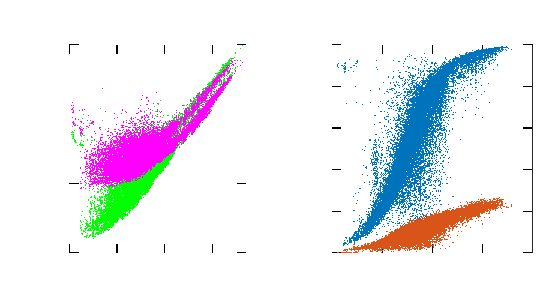
\includegraphics{./figures/experiments/c/time_analysis}}%
    \gplfronttext
  \end{picture}%
\endgroup

  \vspace{0.6cm}
  \caption{\small Left: CBGL's execution time with respect to environment area
           for two choices of overlying scan--to--map-scan matching
           methods. In rough terms $time_{CBGL} \text{ [sec]} =
           17\cdot10^{-3}\cdot area \text{ [} \text{m}^2 \text{]}$.  Right:
           Proportion of CBGL $\circ$ \texttt{x1}'s total execution time spent
           on (a) all operations up to and except for matching, and (b)
           computing map-scans, with respect to area}
  \vspace{-0.5cm}
  \label{fig:c:time_analysis}
\end{figure}
